\chapter{Исследовательский раздел}
\label{cha:research}

В данном разделе описаны эксперименты, проводимые с разработанным программным обеспечением. Эксперименты проводятся с целью определения скоростных характеристик разработанного программного обеспечения и метода в целом, производится оценка точности обнаружения ситуаций гонок в программах в зависимости от их структуры.

\section{Условия проведения экспериментов}

Проведение экспериментов производилось в следующих условиях:
\begin{enumerate}
    \item аппаратное обеспечение:
        \begin{enumerate}
            \item AMD Turion(tm) X2 Ultra Dual-Core Mobile ZM-82 2,2GHz;
            \item 3096 Мб ОЗУ;
        \end{enumerate}
    \item программное обеспечение:
        \begin{enumerate}
            \item ОС Fedora GNU/Linux 20.0 3.11.10-301.fc20.i686;
            \item GCC 4.8.2;
            \item Python 2.7.5;
            \item gcc-python-plugin 0.12.
        \end{enumerate}
\end{enumerate}

\section{Исследование скоростных характеристик}

Для проведения экспериментов по определению скоростных характеристик за основу была взята задача <<читатели-писатели>>. В ней предполагается, что есть некоторый общий для всех потоков ресурс. Часть потоков получает к нему доступ только для чтения, а часть - для записи. При этом чтение может осуществляться одновременно из нескольких потоков. Код анализируемой программы представлен в листинге ~\ref{lst:readers-writers}.

\lstinputlisting[language=C,caption=Код решения задачи "читатели-писатели" (\Code{readers-writers.c}),label=lst:readers-writers]{inc/src/readers-writers.c}

В процессе проведения экспериментов проводилось изменение числа потоков, создаваемых в функции \textbf{main}, и максимального количества вхождений базового блока в анализируемый путь. Графики зависимостей количества анализируемых путей и количества анализируемых инструкций от изменения максимального количества вхождений базового блока в путь представлены на рис.~\ref{fig:graphic1} и на рис.~\ref{fig:graphic2} соответственно. Зависимости времени анализа от количества анализируемых путей, количества потоков и путей представлены на рис.~\ref{fig:graphic3}, рис.~\ref{fig:graphic4} и рис.~\ref{fig:graphic5} соответственно. Видно, что ... (заключение по полученным графикам)

\begin{figure}[h]
  \centering
  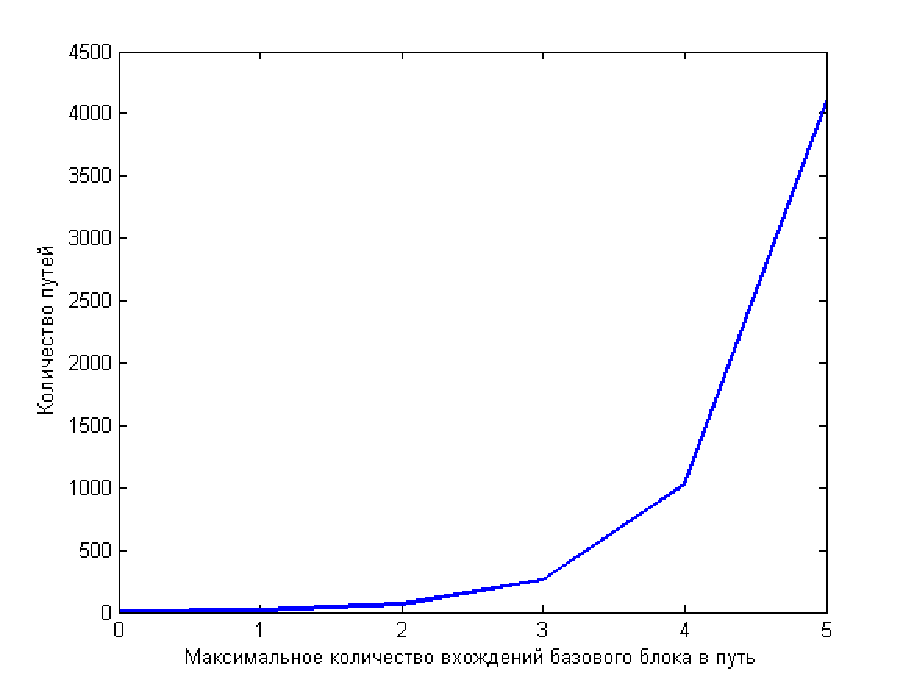
\includegraphics[width=0.9\textwidth]{inc/png/graphic1}
  \caption{Зависимость количества анализируемых путей от максимального количества вхождений базового блока путь}
  \label{fig:graphic1}
\end{figure}

\begin{figure}[h]
  \centering
  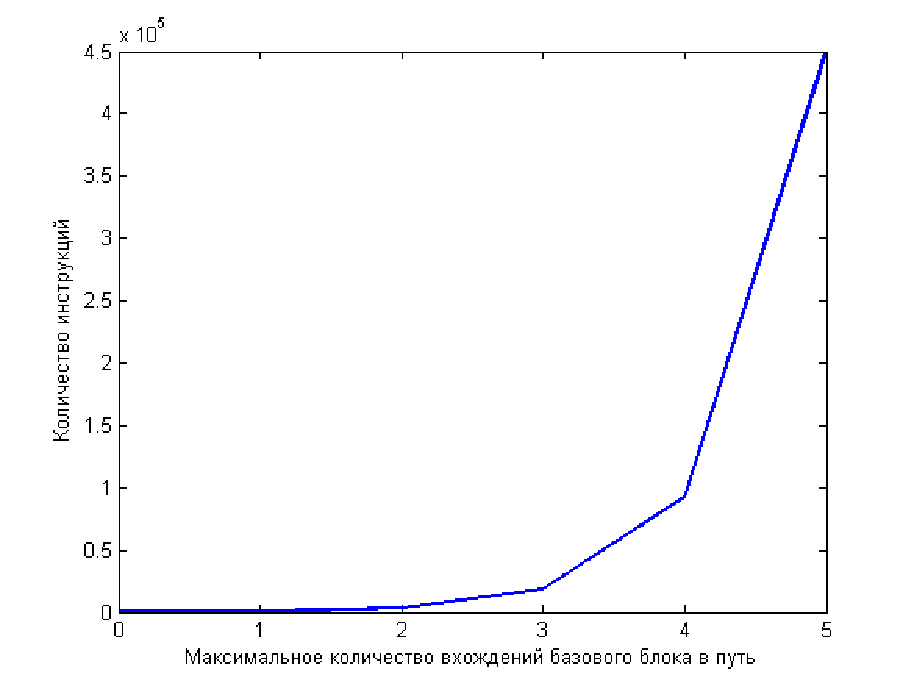
\includegraphics[width=0.9\textwidth]{inc/png/graphic2}
  \caption{Зависимость количества анализируемых инструкций от максимального количества вхождений базового блока путь}
  \label{fig:graphic2}
\end{figure}

\begin{figure}[h]
  \centering
  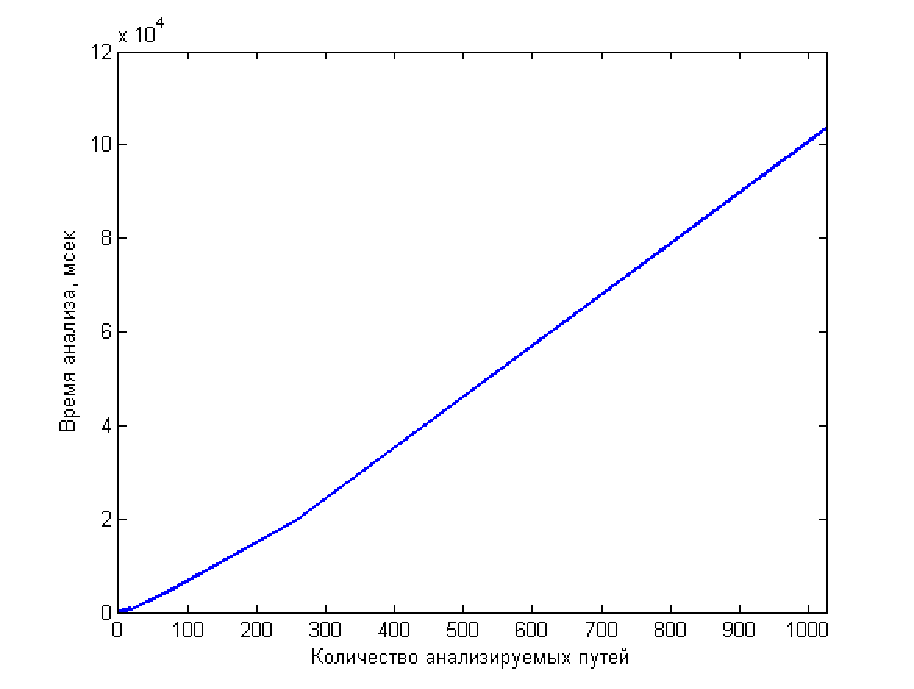
\includegraphics[width=0.9\textwidth]{inc/png/graphic3}
  \caption{Зависимость времени анализа от количества анализируемых путей}
  \label{fig:graphic3}
\end{figure}

\begin{figure}[h]
  \centering
  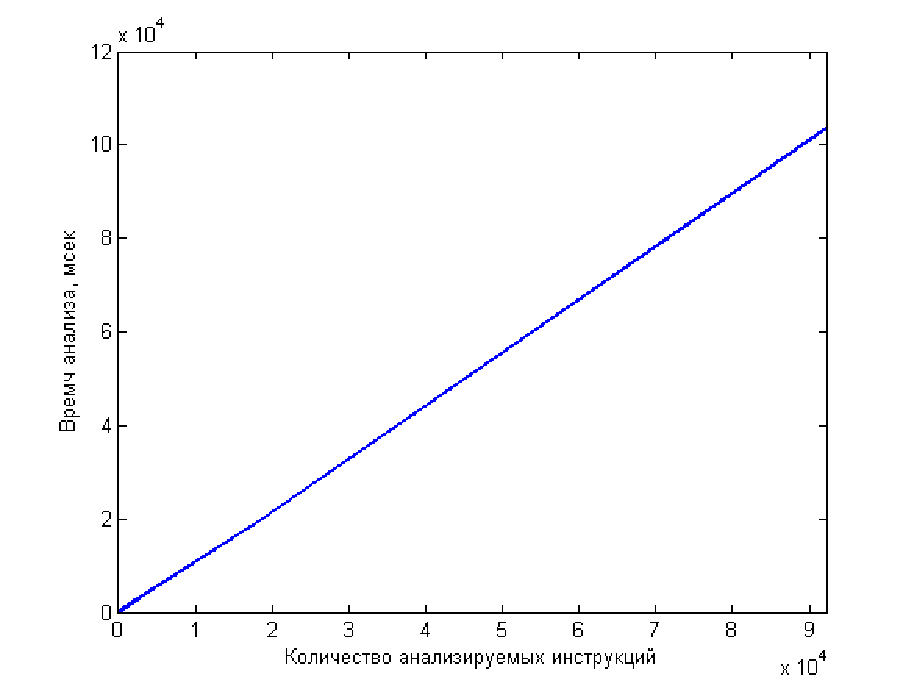
\includegraphics[width=0.9\textwidth]{inc/png/graphic4}
  \caption{Зависимость времени анализа от количества анализируемых инструкций}
  \label{fig:graphic4}
\end{figure}

\begin{figure}[h]
  \centering
  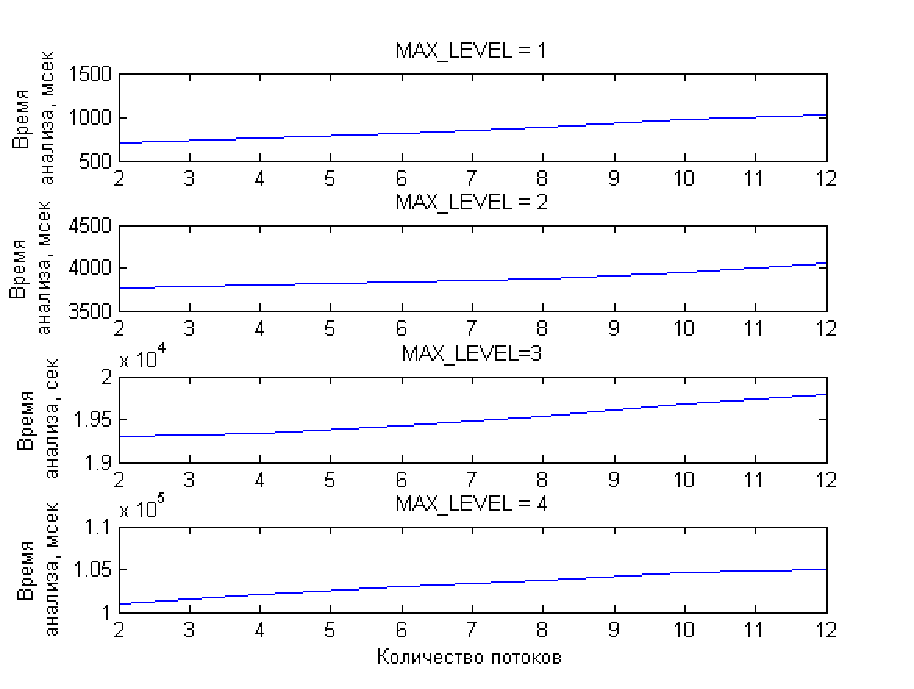
\includegraphics[width=0.9\textwidth]{inc/png/graphic5}
  \caption{Зависимость времени анализа от количества потоков}
  \label{fig:graphic5}
\end{figure}


\section{Исследование точности}

Для исследования точности получаемых результатов использовался тестовый набор программ. Рассмотрим далее результаты полученные на каждом тестовом примере, определим количество правильно обнаруженных ситуаций гонок, количества ошибок первого и второго рода.

\subsection{Программа 1}

Текст программы представлен в листинге~\ref{lst:test1}. В представленной программе в функции \textbf{main} создается 3 потока, в каждом из которых выполняется вызов функции \textbf{munge} с различными параметрами. В тексте программы отсутствуют циклы и ветвления. Анализатор выявил следующие места возникновения гонок:
\begin{verbatim}
WARNING: Race condition when accessing the variable y (global) on line 34
WARNING: Race condition when accessing the variable x (global) on line 34
WARNING: Race condition when accessing the variable z (global) on line 34
WARNING: Race condition when accessing the variable y (global) on line 8
WARNING: Race condition when accessing the variable x (global) on line 8
WARNING: Race condition when accessing the variable z (global) on line 8
\end{verbatim}
Среди найденных анализатором возможных мест возникновения гонок таковыми являются только две:
\begin{verbatim}
WARNING: Race condition when accessing the variable y (global) on line 8
WARNING: Race condition when accessing the variable z (global) on line 8
\end{verbatim}
Остальные обнаруженные места являются ошибочными, и являются ошибками второго рода. Их появление связано с тем, что при разработке метода было сделано предположение о параллельном выполнении всех потоков программы, поэтому, хотя инициализация разделяемых переменных $x$, $y$ и $z$ выполняется в функции \textbf{main} до создания остальных потоков, анализатор показывает место их инициализации, как потенциальное место возникновения гонок.

\lstinputlisting[language=C,caption=Программа 1(\Code{test1.c}),label=lst:test1]{inc/src/test1.c}

\subsection{Программа 2}

Текст программы представлен в листинге~\ref{lst:test2}. В представленной программе в функции \textbf{main} выпоняется создание двух потоков, в каждом из которых производится модификация глобальной переменной $x$. В одном из потоков захват блокировки, доступ к глобальной переменной и освобождение блокировки происходит в случае, когда выполняется определенное условие. Анализатор не выявил мест возникновения гонок:
\begin{verbatim}
OK
\end{verbatim}

\lstinputlisting[language=C,caption=Программа 2(\Code{test2.c}),label=lst:test2]{inc/src/test2.c}

\subsection{Программа 3}

Текст программы представлен в листинге~\ref{lst:test3}. Анализатор не выявил мест возникновения гонок:
\begin{verbatim}
OK
\end{verbatim}

\lstinputlisting[language=C,caption=Программа 3(\Code{test3.c}),label=lst:test3]{inc/src/test3.c}
